\documentclass{standalone}

\usepackage{pgfplots,tikz,amsmath}
\begin{document}
        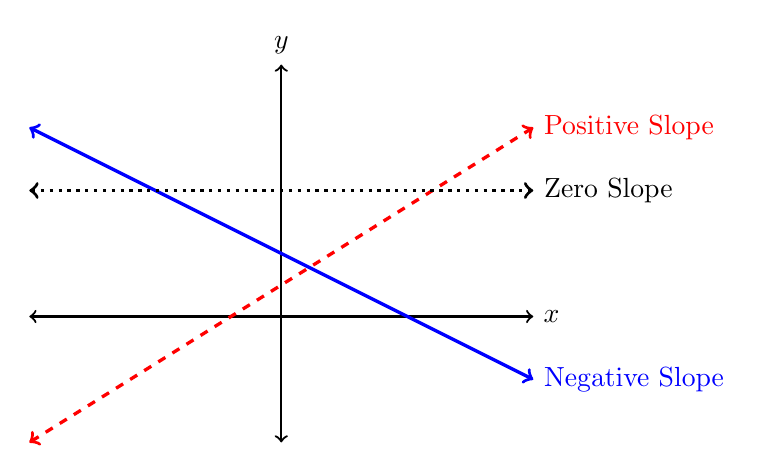
\begin{tikzpicture}[scale=0.8]
            \draw[<->, thick] (-4,0) -- (4,0) node[anchor=west]{$x$};
            \draw[<->, thick] (0,-2) -- (0,4) node[anchor=south]{$y$};
            \draw[<->, very thick, blue] (-4,3) -- (4,-1) node[anchor=west]{Negative
            Slope};
            \draw[<->, very thick, color=red, dashed] (-4,-2) -- (4,3)
            node[anchor=west]{Positive Slope};
            \draw[<->, very thick, color=black, dotted] (-4,2) -- (4,2)
            node[anchor=west]{Zero Slope};
        \end{tikzpicture}
\end{document}
